\chapter{Classification} \label{chap:chap-3}


% add citation for the chapter if it is a reprint


% remove the following and add your chapter text
\section{Introduction}
Classifying the experiments based on the metals and ligands used is explored to further demonstrate the feasibility of using this encoding technique for various machine learning tasks. An important insight to consider is the similarity between voltammetry data and images. After all, each point has a potential and current value, which is similar to an image's RGB values. The main difference is that an image is 2-dimensional while voltammetry data is 1-dimensional. Many previous works have used convolutional neural networks for classification tasks \cite{SHARMA2018377}. Using this as inspiration, the proposed model architecture for voltammetry data classification uses 1-dimensional convolutional layers.  
It is important to note that the dataset used only contains 800 CV datapoints and 200 DPV datapoints for a total of 1000. For training, the dataset was split with 80\% for training, 10\% for validation, and 10\% for testing. 
\section{Model Architecture}
The model consists of several convolutional layers followed by max-poolling layers to encode the data and reduce dimensions. All layers except for the output layer use the ReLU activation function. The output layer is a dense layer with 10 units and softmax activation function. The Adam optimizer and categorical cross-entropy loss are used to train the model. Additionally, the model uses L2 regularization and early stopping to prevent overfitting and ensure smooth convergence. The Glorot uniform initializer is used for weight initialization to facilitate better gradient flow and prevent exploding gradients. 

\begin{figure}[h!]
  \centering
    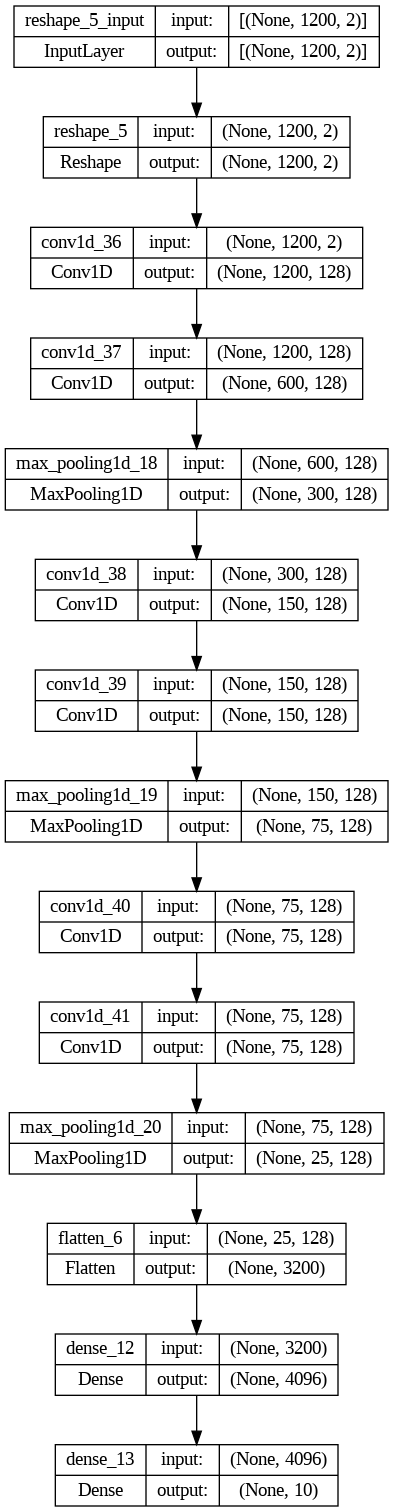
\includegraphics[width=0.25\textwidth]{figures/model_architecture.png}
    \caption{Classification Model Architecture}
    \label{model_arch}
\end{figure}

\section{Results and Discussion}
\begin{center}
\begin{tabular}{c|c}
Model & Accuracy (\%) \\
\hline
CV Ligands & 70.13\% \\
CV Metals & 79.24\% \\
DPV Ligands & 30.00\% \\
DPV Metals & 15.87\%
\end{tabular}
\end{center}
The accuracy of the classifiers were much better for the CV data compared to the DPV data.
\begin{figure}[h!]
  \centering
    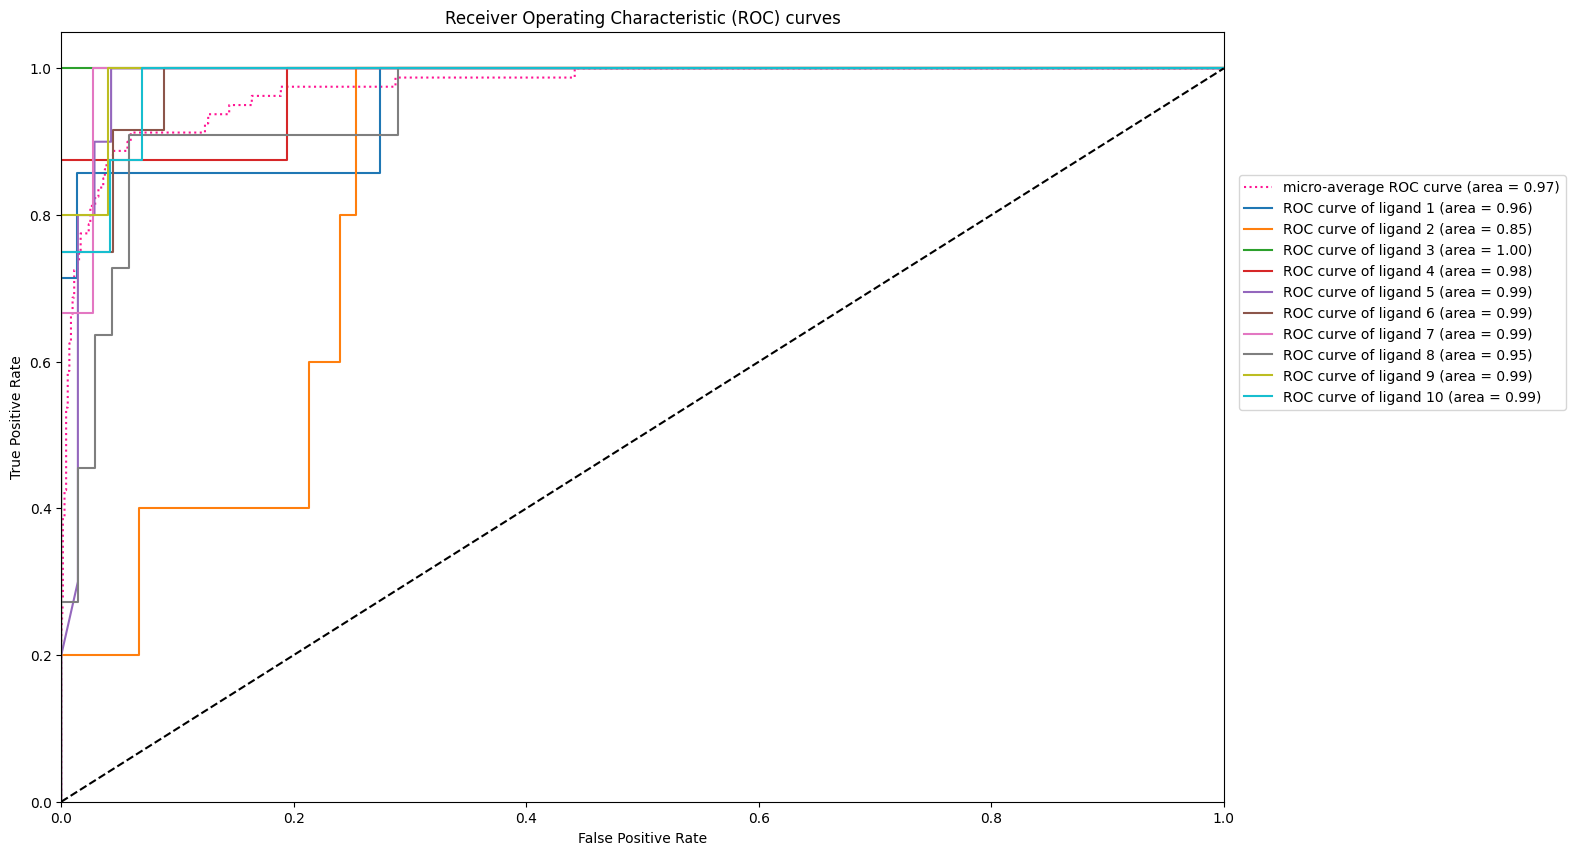
\includegraphics[width=1.0\textwidth]{figures/ligand_roc.png}
    \caption{CV Ligand ROC Curves}
    \label{ligand_roc}
\end{figure}
\begin{figure}[h!]
  \centering
    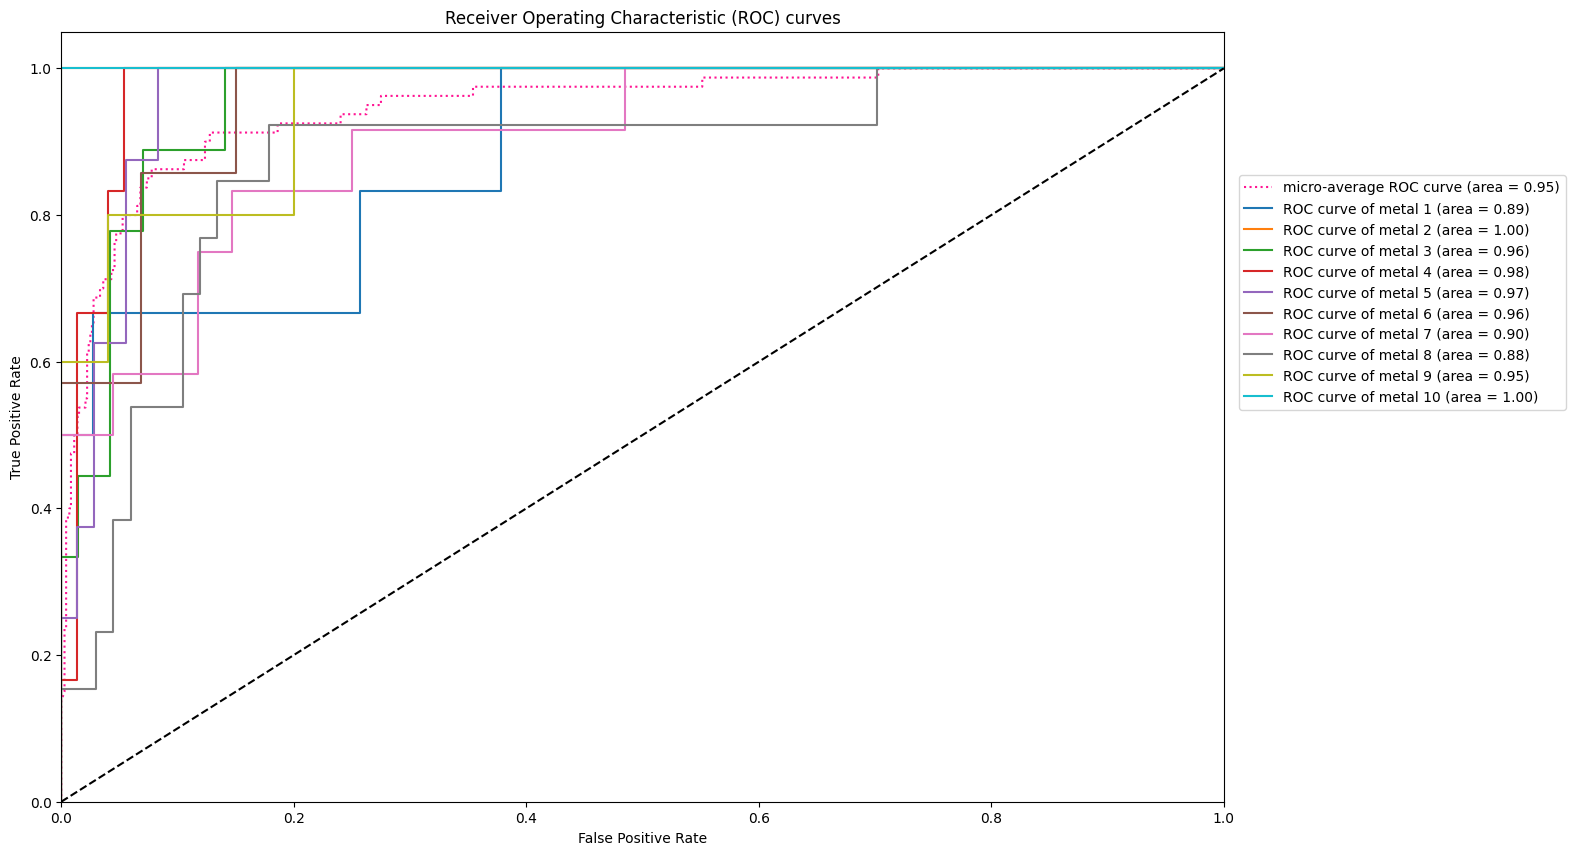
\includegraphics[width=1.0\textwidth]{figures/metal_roc.png}
    \caption{CV Metal ROC Curves}
    \label{metal_roc}
\end{figure}
The area under receiving operating characteristic (ROC) curve shows good results for both metals and ligands. The area under the ROC curve (AUC) calculation summarized the ROC curve analysis into a scalar value, which ranges between 0 and 1. The closer the AUC score to value 1, the better the application’s overall performance.
\begin{figure}[h!]
  \centering
    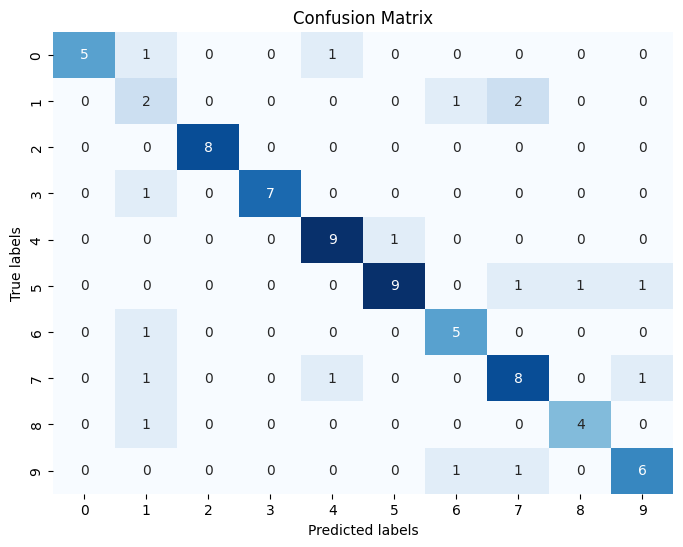
\includegraphics[width=1.0\textwidth]{figures/cv_metal_matrix.png}
    \caption{CV Metal Confusion Matrix}
    \label{cv_metal_matrix}
\end{figure}
From the confusion matrix for metals \ref{cv_metal_matrix}, metal 1 was difficult to recognize with many metals being misclassified as metal 1. 
\begin{figure}[h!]
  \centering
    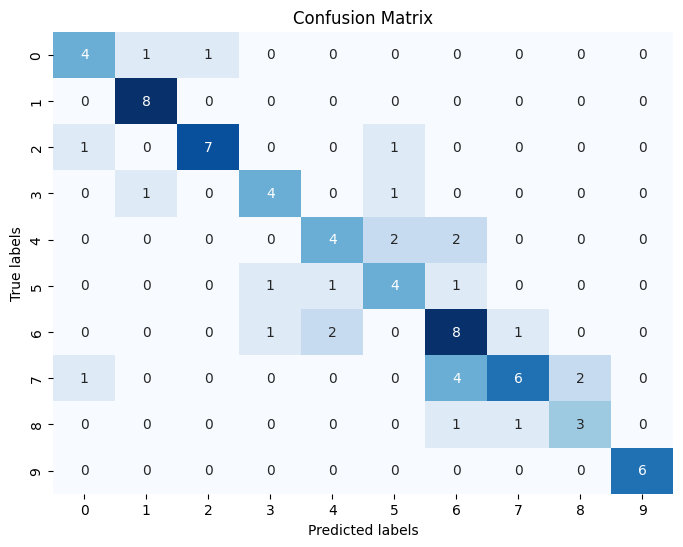
\includegraphics[width=1.0\textwidth]{figures/cv_ligand_matrix.png}
    \caption{CV Ligand Confusion Matrix}
    \label{cv_ligand_matrix}
\end{figure}
From the confusion matrix for ligands \ref{cv_ligand_matrix}, metal 7 was difficult to recognize and was often misclassified as metal 6. 

A major challenge in supervised learning is providing good examples during training. However, despite using a small dataset, these results are promising. 
